\documentclass[]{article}
\usepackage{lmodern}
\usepackage{amssymb,amsmath}
\usepackage{ifxetex,ifluatex}
\usepackage{fixltx2e} % provides \textsubscript
\ifnum 0\ifxetex 1\fi\ifluatex 1\fi=0 % if pdftex
  \usepackage[T1]{fontenc}
  \usepackage[utf8]{inputenc}
\else % if luatex or xelatex
  \ifxetex
    \usepackage{mathspec}
  \else
    \usepackage{fontspec}
  \fi
  \defaultfontfeatures{Ligatures=TeX,Scale=MatchLowercase}
\fi
% use upquote if available, for straight quotes in verbatim environments
\IfFileExists{upquote.sty}{\usepackage{upquote}}{}
% use microtype if available
\IfFileExists{microtype.sty}{%
\usepackage{microtype}
\UseMicrotypeSet[protrusion]{basicmath} % disable protrusion for tt fonts
}{}
\usepackage[margin=1in]{geometry}
\usepackage{hyperref}
\hypersetup{unicode=true,
            pdftitle={razzo pipeline},
            pdfauthor={G. Laudanno and Richel J.C. Bilderbeek},
            pdfborder={0 0 0},
            breaklinks=true}
\urlstyle{same}  % don't use monospace font for urls
\usepackage{color}
\usepackage{fancyvrb}
\newcommand{\VerbBar}{|}
\newcommand{\VERB}{\Verb[commandchars=\\\{\}]}
\DefineVerbatimEnvironment{Highlighting}{Verbatim}{commandchars=\\\{\}}
% Add ',fontsize=\small' for more characters per line
\usepackage{framed}
\definecolor{shadecolor}{RGB}{248,248,248}
\newenvironment{Shaded}{\begin{snugshade}}{\end{snugshade}}
\newcommand{\KeywordTok}[1]{\textcolor[rgb]{0.13,0.29,0.53}{\textbf{#1}}}
\newcommand{\DataTypeTok}[1]{\textcolor[rgb]{0.13,0.29,0.53}{#1}}
\newcommand{\DecValTok}[1]{\textcolor[rgb]{0.00,0.00,0.81}{#1}}
\newcommand{\BaseNTok}[1]{\textcolor[rgb]{0.00,0.00,0.81}{#1}}
\newcommand{\FloatTok}[1]{\textcolor[rgb]{0.00,0.00,0.81}{#1}}
\newcommand{\ConstantTok}[1]{\textcolor[rgb]{0.00,0.00,0.00}{#1}}
\newcommand{\CharTok}[1]{\textcolor[rgb]{0.31,0.60,0.02}{#1}}
\newcommand{\SpecialCharTok}[1]{\textcolor[rgb]{0.00,0.00,0.00}{#1}}
\newcommand{\StringTok}[1]{\textcolor[rgb]{0.31,0.60,0.02}{#1}}
\newcommand{\VerbatimStringTok}[1]{\textcolor[rgb]{0.31,0.60,0.02}{#1}}
\newcommand{\SpecialStringTok}[1]{\textcolor[rgb]{0.31,0.60,0.02}{#1}}
\newcommand{\ImportTok}[1]{#1}
\newcommand{\CommentTok}[1]{\textcolor[rgb]{0.56,0.35,0.01}{\textit{#1}}}
\newcommand{\DocumentationTok}[1]{\textcolor[rgb]{0.56,0.35,0.01}{\textbf{\textit{#1}}}}
\newcommand{\AnnotationTok}[1]{\textcolor[rgb]{0.56,0.35,0.01}{\textbf{\textit{#1}}}}
\newcommand{\CommentVarTok}[1]{\textcolor[rgb]{0.56,0.35,0.01}{\textbf{\textit{#1}}}}
\newcommand{\OtherTok}[1]{\textcolor[rgb]{0.56,0.35,0.01}{#1}}
\newcommand{\FunctionTok}[1]{\textcolor[rgb]{0.00,0.00,0.00}{#1}}
\newcommand{\VariableTok}[1]{\textcolor[rgb]{0.00,0.00,0.00}{#1}}
\newcommand{\ControlFlowTok}[1]{\textcolor[rgb]{0.13,0.29,0.53}{\textbf{#1}}}
\newcommand{\OperatorTok}[1]{\textcolor[rgb]{0.81,0.36,0.00}{\textbf{#1}}}
\newcommand{\BuiltInTok}[1]{#1}
\newcommand{\ExtensionTok}[1]{#1}
\newcommand{\PreprocessorTok}[1]{\textcolor[rgb]{0.56,0.35,0.01}{\textit{#1}}}
\newcommand{\AttributeTok}[1]{\textcolor[rgb]{0.77,0.63,0.00}{#1}}
\newcommand{\RegionMarkerTok}[1]{#1}
\newcommand{\InformationTok}[1]{\textcolor[rgb]{0.56,0.35,0.01}{\textbf{\textit{#1}}}}
\newcommand{\WarningTok}[1]{\textcolor[rgb]{0.56,0.35,0.01}{\textbf{\textit{#1}}}}
\newcommand{\AlertTok}[1]{\textcolor[rgb]{0.94,0.16,0.16}{#1}}
\newcommand{\ErrorTok}[1]{\textcolor[rgb]{0.64,0.00,0.00}{\textbf{#1}}}
\newcommand{\NormalTok}[1]{#1}
\usepackage{graphicx,grffile}
\makeatletter
\def\maxwidth{\ifdim\Gin@nat@width>\linewidth\linewidth\else\Gin@nat@width\fi}
\def\maxheight{\ifdim\Gin@nat@height>\textheight\textheight\else\Gin@nat@height\fi}
\makeatother
% Scale images if necessary, so that they will not overflow the page
% margins by default, and it is still possible to overwrite the defaults
% using explicit options in \includegraphics[width, height, ...]{}
\setkeys{Gin}{width=\maxwidth,height=\maxheight,keepaspectratio}
\IfFileExists{parskip.sty}{%
\usepackage{parskip}
}{% else
\setlength{\parindent}{0pt}
\setlength{\parskip}{6pt plus 2pt minus 1pt}
}
\setlength{\emergencystretch}{3em}  % prevent overfull lines
\providecommand{\tightlist}{%
  \setlength{\itemsep}{0pt}\setlength{\parskip}{0pt}}
\setcounter{secnumdepth}{0}
% Redefines (sub)paragraphs to behave more like sections
\ifx\paragraph\undefined\else
\let\oldparagraph\paragraph
\renewcommand{\paragraph}[1]{\oldparagraph{#1}\mbox{}}
\fi
\ifx\subparagraph\undefined\else
\let\oldsubparagraph\subparagraph
\renewcommand{\subparagraph}[1]{\oldsubparagraph{#1}\mbox{}}
\fi

%%% Use protect on footnotes to avoid problems with footnotes in titles
\let\rmarkdownfootnote\footnote%
\def\footnote{\protect\rmarkdownfootnote}

%%% Change title format to be more compact
\usepackage{titling}

% Create subtitle command for use in maketitle
\newcommand{\subtitle}[1]{
  \posttitle{
    \begin{center}\large#1\end{center}
    }
}

\setlength{\droptitle}{-2em}

  \title{razzo pipeline}
    \pretitle{\vspace{\droptitle}\centering\huge}
  \posttitle{\par}
    \author{G. Laudanno and Richel J.C. Bilderbeek}
    \preauthor{\centering\large\emph}
  \postauthor{\par}
      \predate{\centering\large\emph}
  \postdate{\par}
    \date{2018-10-18}


\begin{document}
\maketitle

Legenda: nLTT = normalized lineages through time; BD = Birth Death
Model; MBD = Multiple Birth Death Model;

This is the pipeline to follow for the Razzo project. Our aim is to
compare two nLTT distributions related to two tree posteriors: one
descending from MBD alignments and another one from BD alignments. Both
posteriors are generated using a BD prior in BEAST.

\begin{Shaded}
\begin{Highlighting}[]
\ControlFlowTok{if}\NormalTok{ (}\OperatorTok{!}\KeywordTok{require}\NormalTok{(mbd)) \{devtools}\OperatorTok{::}\KeywordTok{install_github}\NormalTok{(}\StringTok{"Giappo/mbd"}\NormalTok{)\}}
\end{Highlighting}
\end{Shaded}

\begin{verbatim}
## Loading required package: mbd
\end{verbatim}

\begin{Shaded}
\begin{Highlighting}[]
\ControlFlowTok{if}\NormalTok{ (}\OperatorTok{!}\KeywordTok{require}\NormalTok{(TESS)) \{}
  \KeywordTok{install.packages}\NormalTok{(}\StringTok{"TESS"}\NormalTok{, }\DataTypeTok{repo =} \StringTok{"https://lib.ugent.be/CRAN/"}\NormalTok{)}
\NormalTok{\}}
\end{Highlighting}
\end{Shaded}

\begin{verbatim}
## Loading required package: TESS
\end{verbatim}

\begin{verbatim}
## Loading required package: ape
\end{verbatim}

\begin{verbatim}
## Loading required package: coda
\end{verbatim}

\begin{verbatim}
## Loading required package: deSolve
\end{verbatim}

\begin{Shaded}
\begin{Highlighting}[]
\ControlFlowTok{if}\NormalTok{ (}\OperatorTok{!}\KeywordTok{require}\NormalTok{(pirouette)) \{}
\NormalTok{  devtools}\OperatorTok{::}\KeywordTok{install_github}\NormalTok{(}\StringTok{"richelbilderbeek/babette"}\NormalTok{)}
\NormalTok{  devtools}\OperatorTok{::}\KeywordTok{install_github}\NormalTok{(}\StringTok{"richelbilderbeek/pirouette"}\NormalTok{)}
\NormalTok{\}}
\end{Highlighting}
\end{Shaded}

\begin{verbatim}
## Loading required package: pirouette
\end{verbatim}

\subsection{Folder structure}\label{folder-structure}

In \texttt{folder\_name}:

\begin{itemize}
\tightlist
\item
  \texttt{1}

  \begin{itemize}
  \tightlist
  \item
    \texttt{parameters.csv}: the parameter file, created by
    \texttt{raz\_create\_parameter\_files}
  \item
    \texttt{mbd.tree}: the true MBD tree, created by
    \texttt{raz\_create\_input\_files}
  \item
    \texttt{mbd.fasta}: the true MBD alignment, created by
    \texttt{raz\_create\_input\_files}
  \item
    \texttt{bd.tree}: the twin BD tree, created by
    \texttt{raz\_create\_input\_files}
  \item
    \texttt{bd.fasta}: the twin BD alignment, created by
    \texttt{raz\_create\_input\_files}
  \item
    \texttt{mbd.trees}: the posterior trees from \texttt{mbd.tree},
    created by \texttt{raz\_create\_inference\_files("mbd.tree")}
  \item
    \texttt{mbd.log}: the posterior parameter estimates from
    \texttt{mbd.tree}, created by
    \texttt{raz\_create\_inference\_files("mbd.tree")}
  \item
    \texttt{mbd\_mar\_lik.csv}: the posterior's marginal likelihood from
    \texttt{mbd.tree}, created by
    \texttt{raz\_create\_inference\_files("mbd.tree")}
  \item
    \texttt{bd.trees}: the posterior trees from \texttt{bd.tree},
    created by \texttt{raz\_create\_inference\_files("bd.tree")}
  \item
    \texttt{bd.log}: the posterior parameter estimates from
    \texttt{bd.tree}, created by
    \texttt{raz\_create\_inference\_files("bd.tree")}
  \item
    \texttt{bd\_mar\_lik.csv}: the posterior's marginal likelihood from
    \texttt{bd.tree}, created by
    \texttt{raz\_create\_inference\_files("bd.tree")}
  \item
    \texttt{mbd\_nltts.csv}: the nLTT statistic distribution between
    \texttt{mbd.tree} and \texttt{mbd.trees}, created by
    \texttt{raz\_create\_nltt\_file("mbd.tree",\ "mbd.trees")}
  \item
    \texttt{bd\_nltts.csv}: the nLTT statistic distribution between
    \texttt{bd.tree} and \texttt{bd.trees}, created by
    \texttt{raz\_create\_nltt\_file("bd.tree",\ "bd.trees")}
  \end{itemize}
\item
  \texttt{2}
\item
  \texttt{3}
\item
  Etcetera
\end{itemize}

\subsection{Overview}\label{overview}

\begin{figure}
\centering
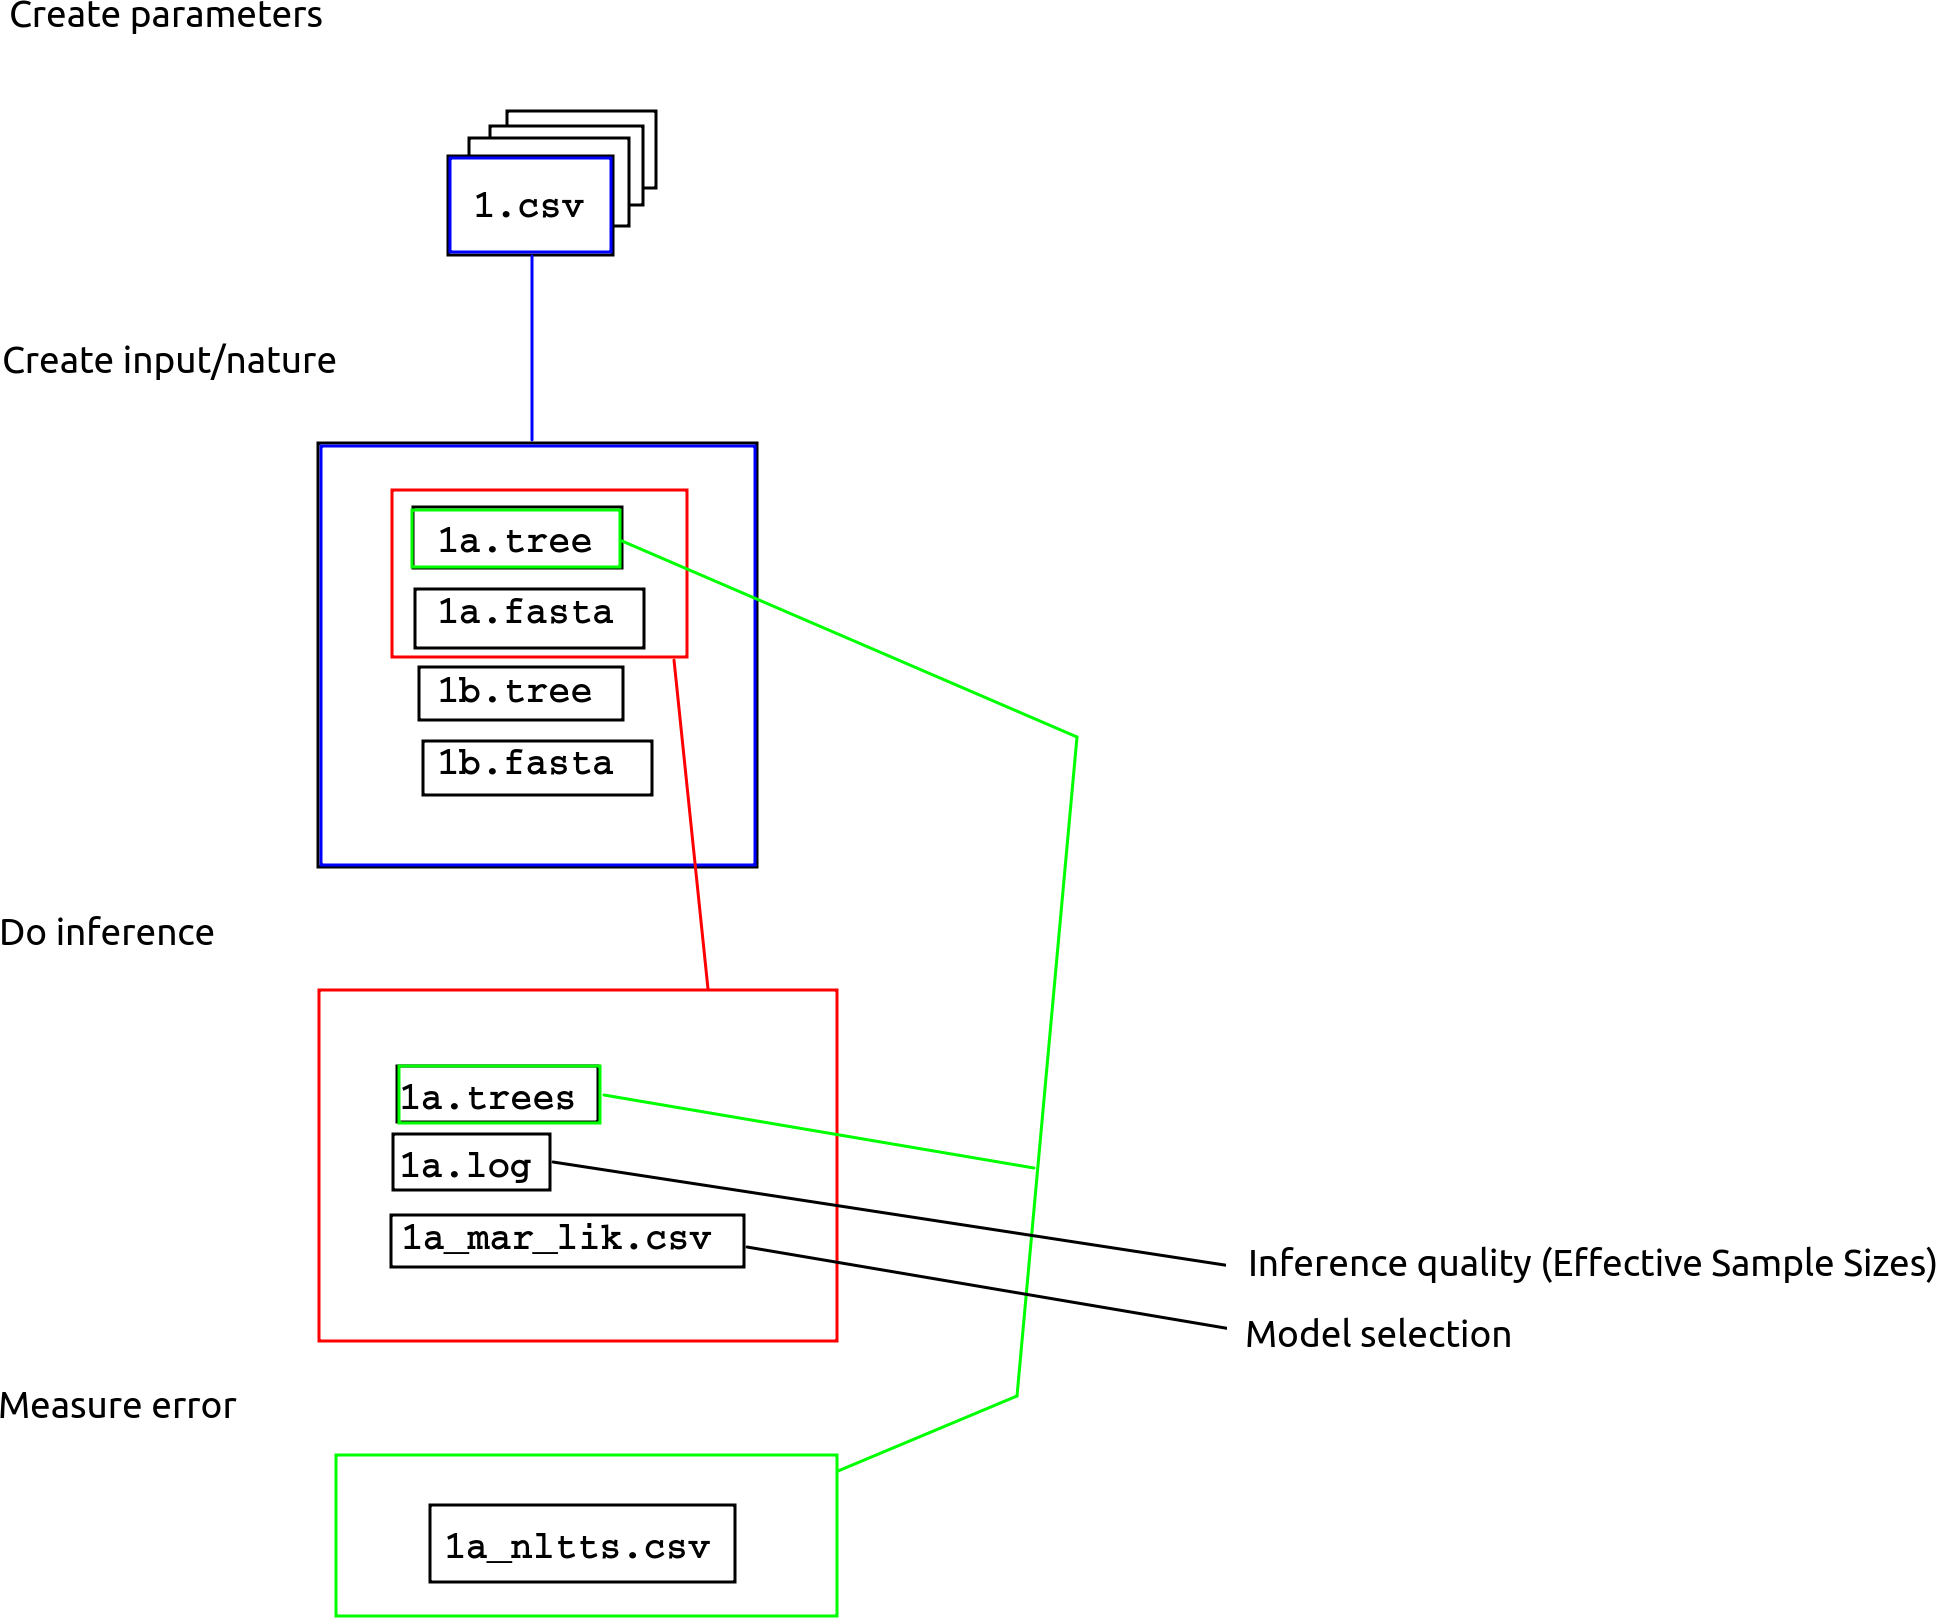
\includegraphics{pipeline.png}
\caption{Pipeline}
\end{figure}

Load the library:

\begin{Shaded}
\begin{Highlighting}[]
\KeywordTok{library}\NormalTok{(razzo)}
\end{Highlighting}
\end{Shaded}

We will work in this folder:

\begin{Shaded}
\begin{Highlighting}[]
\NormalTok{folder_name <-}\StringTok{ }\KeywordTok{tempdir}\NormalTok{()}
\end{Highlighting}
\end{Shaded}

\subsection{Step 0: create parameters}\label{step-0-create-parameters}

\section{Create all parameter files}\label{create-all-parameter-files}

\section{parameters\_filenames \textless{}-
raz\_create\_parameters\_files()}\label{parameters_filenames---raz_create_parameters_files}

\section{\texorpdfstring{testit::assert(``1.csv'' \%in\%
parameters\_filenames)}{testit::assert(1.csv \%in\% parameters\_filenames)}}\label{testitassert1.csv-in-parameters_filenames}

\section{}\label{section}

\section{\# Create all true trees, true alignments and their
twins}\label{create-all-true-trees-true-alignments-and-their-twins}

\section{for (parameters\_filename in parameters\_filenames)
\{}\label{for-parameters_filename-in-parameters_filenames}

\section{input\_filenames \textless{}-
raz\_create\_input\_files(parameters\_filename)}\label{input_filenames---raz_create_input_filesparameters_filename}

\section{\# True MBD tree}\label{true-mbd-tree}

\section{\texorpdfstring{testit::assert(``1a.tree'' \%in\%
input\_filenames)}{testit::assert(1a.tree \%in\% input\_filenames)}}\label{testitassert1a.tree-in-input_filenames}

\section{\# True MBD alignment}\label{true-mbd-alignment}

\section{\texorpdfstring{testit::assert(``1a.fasta'' \%in\%
input\_filenames)}{testit::assert(1a.fasta \%in\% input\_filenames)}}\label{testitassert1a.fasta-in-input_filenames}

\section{\# Twin BD tree}\label{twin-bd-tree}

\section{\texorpdfstring{testit::assert(``1b.tree'' \%in\%
input\_filenames)}{testit::assert(1b.tree \%in\% input\_filenames)}}\label{testitassert1b.tree-in-input_filenames}

\section{\# Twin BD alignment}\label{twin-bd-alignment}

\section{\texorpdfstring{testit::assert(``1b.fasta'' \%in\%
input\_filenames)}{testit::assert(1b.fasta \%in\% input\_filenames)}}\label{testitassert1b.fasta-in-input_filenames}

\section{\}}\label{section-1}

\section{}\label{section-2}

\section{\# Do the inference}\label{do-the-inference}

\section{\texorpdfstring{fasta\_filenames \textless{}- c(``1a.fasta'')
\# Search the
folder}{fasta\_filenames \textless{}- c(1a.fasta) \# Search the folder}}\label{fasta_filenames---c1a.fasta-search-the-folder}

\section{for (fasta\_filename in
fasta\_filenames)}\label{for-fasta_filename-in-fasta_filenames}

\section{\{}\label{section-3}

\section{output\_filenames \textless{}-
raz\_create\_inference\_files(fasta\_filename)}\label{output_filenames---raz_create_inference_filesfasta_filename}

\section{\# Posterior trees}\label{posterior-trees}

\section{\texorpdfstring{testit::assert(``1a.trees'' \%in\%
output\_filenames)}{testit::assert(1a.trees \%in\% output\_filenames)}}\label{testitassert1a.trees-in-output_filenames}

\section{\# Trace of MCMC, to estimate the Effective Sample
Sizes}\label{trace-of-mcmc-to-estimate-the-effective-sample-sizes}

\section{\texorpdfstring{testit::assert(``1a.log'' \%in\%
output\_filenames)}{testit::assert(1a.log \%in\% output\_filenames)}}\label{testitassert1a.log-in-output_filenames}

\section{\# Marginal likelihood}\label{marginal-likelihood}

\section{\texorpdfstring{testit::assert(``1a\_mar\_lik.csv'' \%in\%
output\_filenames)}{testit::assert(1a\_mar\_lik.csv \%in\% output\_filenames)}}\label{testitassert1a_mar_lik.csv-in-output_filenames}

\section{\}}\label{section-4}

\section{}\label{section-5}

\section{\# Create the nLTT
distribution}\label{create-the-nltt-distribution}

\section{\texorpdfstring{trees\_filenames \textless{}- c(``1a.trees'')
\# Search the
folder}{trees\_filenames \textless{}- c(1a.trees) \# Search the folder}}\label{trees_filenames---c1a.trees-search-the-folder}

\section{for (trees\_filename in
trees\_filenames)}\label{for-trees_filename-in-trees_filenames}

\section{\{}\label{section-6}

\section{nltt\_filename \textless{}-
raz\_create\_nltt\_file(trees\_filename)}\label{nltt_filename---raz_create_nltt_filetrees_filename}

\section{\texorpdfstring{testit::assert(``1a\_nltts.csv'' \%in\%
nltt\_filename)}{testit::assert(1a\_nltts.csv \%in\% nltt\_filename)}}\label{testitassert1a_nltts.csv-in-nltt_filename}

\section{\}}\label{section-7}

\section{}\label{section-8}

\section{\# All files are in place!}\label{all-files-are-in-place}

Here we create all parameter files:

\begin{Shaded}
\begin{Highlighting}[]
\ControlFlowTok{if}\NormalTok{ (}\DecValTok{1} \OperatorTok{==}\StringTok{ }\DecValTok{2}\NormalTok{) \{}
\NormalTok{  parameters_filenames <-}\StringTok{ }\KeywordTok{raz_create_parameters_files}\NormalTok{(folder_name)}
\NormalTok{  testit}\OperatorTok{::}\KeywordTok{assert}\NormalTok{(}\KeywordTok{file.path}\NormalTok{(folder_name, }\StringTok{"1"}\NormalTok{, }\StringTok{"parameters.csv"}\NormalTok{) }\OperatorTok\StringTok{ }\NormalTok{parameters_filenames)}
\NormalTok{\}}
\end{Highlighting}
\end{Shaded}

\subsection{Step 1: create input files}\label{step-1-create-input-files}

Each parameter file is read to create a MBD tree and alignment and its
BD twin:

\begin{Shaded}
\begin{Highlighting}[]
\ControlFlowTok{if}\NormalTok{ (}\DecValTok{1} \OperatorTok{==}\StringTok{ }\DecValTok{2}\NormalTok{) \{}
  \CommentTok{# Create all true trees, true alignments and their twins}
  \ControlFlowTok{for}\NormalTok{ (parameters_filename }\ControlFlowTok{in}\NormalTok{ parameters_filenames) \{}
\NormalTok{    input_filenames <-}\StringTok{ }\KeywordTok{raz_create_input_files}\NormalTok{(parameters_filename)}
    \CommentTok{# True MBD tree}
\NormalTok{    testit}\OperatorTok{::}\KeywordTok{assert}\NormalTok{(}\KeywordTok{file.path}\NormalTok{(folder_name, }\StringTok{"1"}\NormalTok{, }\StringTok{"mbd.tree"}\NormalTok{) }\OperatorTok\StringTok{ }\NormalTok{input_filenames)}
    \CommentTok{# True MBD alignment}
\NormalTok{    testit}\OperatorTok{::}\KeywordTok{assert}\NormalTok{(}\KeywordTok{file.path}\NormalTok{(folder_name, }\StringTok{"1"}\NormalTok{, }\StringTok{"mbd.fasta"}\NormalTok{) }\OperatorTok\StringTok{ }\NormalTok{input_filenames)}
    \CommentTok{# Twin BD tree}
\NormalTok{    testit}\OperatorTok{::}\KeywordTok{assert}\NormalTok{(}\KeywordTok{file.path}\NormalTok{(folder_name, }\StringTok{"1"}\NormalTok{, }\StringTok{"bd.tree"}\NormalTok{) }\OperatorTok\StringTok{ }\NormalTok{input_filenames)}
    \CommentTok{# Twin BD alignment}
\NormalTok{    testit}\OperatorTok{::}\KeywordTok{assert}\NormalTok{(}\KeywordTok{file.path}\NormalTok{(folder_name, }\StringTok{"1"}\NormalTok{, }\StringTok{"bd.fasta"}\NormalTok{) }\OperatorTok\StringTok{ }\NormalTok{input_filenames)}
\NormalTok{  \}}
\NormalTok{\}}
\end{Highlighting}
\end{Shaded}

Show the first MBD tree:

\begin{Shaded}
\begin{Highlighting}[]
\CommentTok{# }\AlertTok{TODO}\CommentTok{: Issue #8: actually create an MBD tree and save it}
\ControlFlowTok{if}\NormalTok{ (}\DecValTok{1} \OperatorTok{==}\StringTok{ }\DecValTok{2}\NormalTok{) \{}
  \KeywordTok{plot}\NormalTok{(}\KeywordTok{file.path}\NormalTok{(folder_name, }\StringTok{"1"}\NormalTok{, }\StringTok{"mbd.tree"}\NormalTok{))}
\NormalTok{\}}
\end{Highlighting}
\end{Shaded}

Then we want to generate a ``twin'' BD tree. To create such tree we have
to estimate the best lambda and mu to make the comparison fair. To
estimate the parameters we run a ML inference using the BD model. We
also want to condition on the same amount of tips and on the survival of
the phylogeny (cond = 2).

\begin{Shaded}
\begin{Highlighting}[]
\ControlFlowTok{if}\NormalTok{ (}\DecValTok{1} \OperatorTok{==}\StringTok{ }\DecValTok{2}\NormalTok{) \{}
  \KeywordTok{plot}\NormalTok{(}\KeywordTok{file.path}\NormalTok{(folder_name, }\StringTok{"1"}\NormalTok{, }\StringTok{"bd.tree"}\NormalTok{))}
\NormalTok{\}}
\end{Highlighting}
\end{Shaded}

\subsection{Step 2: create inference
files}\label{step-2-create-inference-files}

\begin{Shaded}
\begin{Highlighting}[]
\ControlFlowTok{if}\NormalTok{ (}\DecValTok{1} \OperatorTok{==}\StringTok{ }\DecValTok{2}\NormalTok{) \{}
  \CommentTok{# Do the inference}
\NormalTok{  fasta_filenames <-}\StringTok{ }\KeywordTok{c}\NormalTok{(}\StringTok{"1a.fasta"}\NormalTok{) }\CommentTok{# Search the folder}
  \ControlFlowTok{for}\NormalTok{ (fasta_filename }\ControlFlowTok{in}\NormalTok{ fasta_filenames) }
\NormalTok{  \{}
\NormalTok{    output_filenames <-}\StringTok{ }\KeywordTok{raz_create_inference_files}\NormalTok{(fasta_filename)}
    \CommentTok{# Posterior trees}
\NormalTok{    testit}\OperatorTok{::}\KeywordTok{assert}\NormalTok{(}\StringTok{"1a.trees"} \OperatorTok\StringTok{ }\NormalTok{output_filenames)}
    \CommentTok{# Trace of MCMC, to estimate the Effective Sample Sizes}
\NormalTok{    testit}\OperatorTok{::}\KeywordTok{assert}\NormalTok{(}\StringTok{"1a.log"} \OperatorTok\StringTok{ }\NormalTok{output_filenames)}
    \CommentTok{# Marginal likelihood}
\NormalTok{    testit}\OperatorTok{::}\KeywordTok{assert}\NormalTok{(}\StringTok{"1a_mar_lik.csv"} \OperatorTok\StringTok{ }\NormalTok{output_filenames)}
\NormalTok{  \}}
\NormalTok{\}}
\end{Highlighting}
\end{Shaded}

\subsection{step 6: calculating nLTT statistics for MBD and
BD}\label{step-6-calculating-nltt-statistics-for-mbd-and-bd}

Finally we calculate the nLTT statistics for both posteriors related to
the original trees.

\begin{Shaded}
\begin{Highlighting}[]
\ControlFlowTok{if}\NormalTok{ (}\DecValTok{1} \OperatorTok{==}\StringTok{ }\DecValTok{2}\NormalTok{) \{}
  \CommentTok{# Create the nLTT distribution}
\NormalTok{  trees_filenames <-}\StringTok{ }\KeywordTok{c}\NormalTok{(}\StringTok{"1a.trees"}\NormalTok{) }\CommentTok{# Search the folder}
  \ControlFlowTok{for}\NormalTok{ (trees_filename }\ControlFlowTok{in}\NormalTok{ trees_filenames)}
\NormalTok{  \{}
    \ControlFlowTok{if}\NormalTok{ (}\DecValTok{1} \OperatorTok{==}\StringTok{ }\DecValTok{2}\NormalTok{) \{}
      \CommentTok{# }\AlertTok{TODO}\CommentTok{: Issue 5}
\NormalTok{      nltt_filename <-}\StringTok{ }\KeywordTok{raz_create_nltt_file}\NormalTok{(trees_filename)}
\NormalTok{      testit}\OperatorTok{::}\KeywordTok{assert}\NormalTok{(}\StringTok{"1a_nltts.csv"} \OperatorTok\StringTok{ }\NormalTok{nltt_filename)}
\NormalTok{    \}}
\NormalTok{  \}}
\NormalTok{\}}
\CommentTok{# All files are in place!}
\end{Highlighting}
\end{Shaded}

\begin{Shaded}
\begin{Highlighting}[]
\CommentTok{# }\AlertTok{TODO}\CommentTok{: plot the nLTT}
\end{Highlighting}
\end{Shaded}

\subsubsection{step 3: simulate the twin BD
tree}\label{step-3-simulate-the-twin-bd-tree}

\subsubsection{(check if the method to keep the topology is right. from
the figures it seems ok-ish. check with small
tree)}\label{check-if-the-method-to-keep-the-topology-is-right.-from-the-figures-it-seems-ok-ish.-check-with-small-tree}

Now that we have the BD equivalent parameters for a fair ``twinning'' we
can simulate a BD tree. We use ``TESS::tess.sim.taxa.age'' to generate
the branching times (BD\_brts). We then plug these branching times in
the l\_table coming from the original MBD tree to be sure that the
topology is the same.

\subsubsection{step 4: generate MBD posterior, given BD
prior}\label{step-4-generate-mbd-posterior-given-bd-prior}

The next step is to use the package ``pirouette'' to generate, from the
MBD tree, first the alignments and then, through BEAST, a posterior
distribution of trees. These trees are obtained using a BD prior. This
means that there are no simultaneous branching events.

\subsubsection{step 5: generate BD posterior, given BD
prior}\label{step-5-generate-bd-posterior-given-bd-prior}

\subsubsection{(check BD\_substitution rate, see Rampal's
email)}\label{check-bd_substitution-rate-see-rampals-email}

We repeat the same process for the tree simulated according to the BD
model. We want to have, in principle, the same amount of substitutions;
to do so we modify the mutation rate according to the ratio of the total
branch lenghts of the trees simulated with the two models.

\begin{Shaded}
\begin{Highlighting}[]
\ControlFlowTok{if}\NormalTok{ (}\DecValTok{1} \OperatorTok{==}\StringTok{ }\DecValTok{2}\NormalTok{) \{}
  
  \KeywordTok{par}\NormalTok{(}\DataTypeTok{mfrow =} \KeywordTok{c}\NormalTok{(}\DecValTok{1}\NormalTok{,}\DecValTok{2}\NormalTok{))}
  \KeywordTok{hist}\NormalTok{(}\KeywordTok{unlist}\NormalTok{(MBD_df.nLTT), }\DataTypeTok{main =} \StringTok{"MBD nLTT"}\NormalTok{)}
  \KeywordTok{hist}\NormalTok{(}\KeywordTok{unlist}\NormalTok{(BD_df.nLTT), }\DataTypeTok{main =} \StringTok{"BD nLTT"}\NormalTok{)}
  \KeywordTok{cat}\NormalTok{(}\StringTok{"Average nLTT for MBD"}\NormalTok{, MBD_mean.nLTT, }\StringTok{"}\CharTok{\textbackslash{}n}\StringTok{Average nLTT for BD "}\NormalTok{, BD_mean.nLTT)}
\NormalTok{\}}
\end{Highlighting}
\end{Shaded}


\end{document}
